%% In the documentclass line, replace "noanswers" with "answers" to view the key.

\documentclass[noanswers]{exam}
\usepackage[utf8]{inputenc}

\title{Chapter 12 Practice Problems}
\author{Section 12.2}
\date{STAT 2300}

\usepackage[bottom=2.2cm, left=2.2cm, right=2.2cm, top=2.2cm]{geometry}
%\usepackage[paperheight=11in, paperwidth=17in, margin=1in]{geometry}
\usepackage{dsfont}
\usepackage{amsmath}
\usepackage{amssymb}
\usepackage{amsthm}
\usepackage{array}
\usepackage{stmaryrd}
\usepackage{pgfplots}
\pgfplotsset{width=10cm,compat=1.9}
\usepackage{multicol}
\setlength{\columnsep}{1in}
\usepackage{nicefrac}

\usepackage{multirow}
\usepackage{enumitem}[shortlabels]
\usepackage{tabu}
\definecolor{purp}{RGB}{102,0,204}
\usepackage{tabularx}
\newcolumntype{C}{>{\centering\arraybackslash $}X<{$}}
\usepackage{wrapfig}
\usepackage[export]{adjustbox}


\makeatletter
\pagestyle{headandfoot}
\firstpageheader{\@date}{\@title}{\@author}
\firstpageheadrule
\runningfootrule
\runningfooter{}{\thepage\ / \numpages}{\@title}
\makeatother

\newcommand{\abs}[1]{\left|#1\right|}
\newcommand{\mat}[4]{\left( \begin{tabular}{>{$}c<{$} >{$}c<{$}} #1&#2 \\ #3&#4 \end{tabular} \right)}
\newcommand{\msc}[1]{\mathds{#1}}
\newcommand{\Z}{\mathds{Z}}
\newcommand{\R}{\mathds{R}}
\newcommand{\N}{\mathds{N}}
\newcommand{\Q}{\mathds{Q}}
\newcommand{\C}{\mathds{C}}
\newcommand{\so}{\implies}
\newcommand{\set}[2]{\left\{ #1 \:|\: #2 \right\}}
\newcommand{\bso}{\Longleftarrow}
\newcommand{\ra}{\rightarrow}
\newcommand{\gen}[1]{\left\langle #1 \right\rangle}
\newcommand{\olin}[1]{\overline{#1}}
\newcommand{\Img}[1]{\text{Im}\left(#1\right)}
\newcommand{\llra}{\longleftrightarrow}
\newcommand{\lra}{\longrightarrow}
\newcommand{\xra}[1]{\xrightarrow{#1}}
\newcommand{\wo}{\setminus}
\newcommand{\mcal}[1]{\mathcal{#1}}
\newcommand{\Aut}[1]{\text{Aut}\left(#1\right)}
\newcommand{\Inn}[1]{\text{Inn}\left(#1\right)}
\newcommand{\syl}[2]{\text{Syl}_{#1}(#2)}
\newcommand{\norm}[1]{\left\|#1\right\|}
\newcommand{\infnorm}[1]{\left\|#1\right\|_{\infty}}
\newcommand{\xn}{\{x_n\}}
\newcommand{\sig}{\sigma}
\newcommand{\id}{\text{id}}
\newcommand{\ep}{\epsilon}
\newcommand{\st}{\text{ s.t. }}
\newcommand{\ran}[1]{\text{Ran}(#1)}
\newcommand{\nCr}[2]{\binom{#1}{#2}}
\newcommand{\Exr}[1]{\paragraph{Exercise #1:}}
\newcommand{\pg}{\paragraph{}}
\newcommand{\ulin}[1]{\underline{#1}}
\newcommand{\tc}[1]{\textcolor{purp}{#1}}

% Solution Specs
\unframedsolutions
\renewcommand{\solutiontitle}{}
\SolutionEmphasis{\color{purp}}
\CorrectChoiceEmphasis{\color{purp}\bfseries}
\setlength\fillinlinelength{0in}

%\begin{solution}[\stretch{1}]
%	hurp durp flurp
%\end{solution}

%\pagestyle{empty}

\renewcommand{\arraystretch}{1.25}
\usepackage{cancel}

\usepackage{scalerel}

\begin{document}

%\noindent\begin{tabular}{@{}p{.3in}p{3in}@{}}
%Name: & \hrulefill
%\end{tabular}
%
%\vspace{2mm}

\noindent Use JMP to answer the following questions. Instructions for how to find the relevant JMP output are included in Chapter 12 of your Lecture Guide.

\begin{questions} 

\question The following data on gender and highest earned degree were collected for individuals with a college degree in the United States. A researcher wonders if there is an association between gender and highest degree earned. Conduct a $\chi^2$ test of independence at the $\alpha=0.05$ level to investigate the researcher's hypothesis.

\begin{center}
\begin{tabular}{|c|c|c|c|c||c|}
\hline
 & \textbf{Bachelor's} & \textbf{Master's} & \textbf{Professional} & \textbf{Doctorate} & \textbf{Total} \\
 \hline
 \textbf{Women} & 644 & 230 & 32 & 18 & 924\\
 \hline
 \textbf{Men} & 506 & 154 & 40 & 26 & 726 \\
 \hline
 \hline
 \textbf{Total} & 1150 & 384 & 72 & 44 & 1650 \\
 \hline
\end{tabular}
\end{center}

\vspace{2mm}

\begin{parts}

\part State the appropriate \textbf{hypotheses} in this context.

\begin{solution}[\stretch{1}]

\vspace{3mm}

$H_0$: Gender and highest degree earned are independent (not associated)

$H_1$: Gender and highest degree earned are dependent (associated)

\vspace{3mm}

\end{solution}

\part What is the \textbf{expected count} for women with a master's degree?

\begin{solution}[\stretch{1}]

\vspace{3mm}

$E=\displaystyle\frac{\text{Row Total}\times\text{Column Total}}{\text{Total Sample Size}}=\frac{924\times 384}{1650}=215.04$

\vspace{3mm}

\end{solution}

\part Are the \textbf{conditions} for the chi-square test of independence of gender and highest degree earned met?

\begin{solution}[\stretch{1}]

\vspace{3mm}

Yes, because all expected counts are greater than 5.

\vspace{3mm}

\end{solution}

\part Calculate the chi-square \textbf{test statistic}.

\begin{solution}[\stretch{1}]

\vspace{3mm}

$E=\displaystyle\frac{(506-506)^2}{506}+\dots+\frac{(32-40.32)^2}{40.32}=10.334$ (from output)

\vspace{3mm}

\end{solution}

\part Find the \textbf{approximate p-value} using the chi-square table. Include a sketch.

\begin{solution}[\stretch{1}]

\vspace{3mm}

$df=(r-1)(c-1)=(2-1)(4-1)=(1)(3)=3$  \hspace{20mm} $0.01<\text{p-value}<0.025$

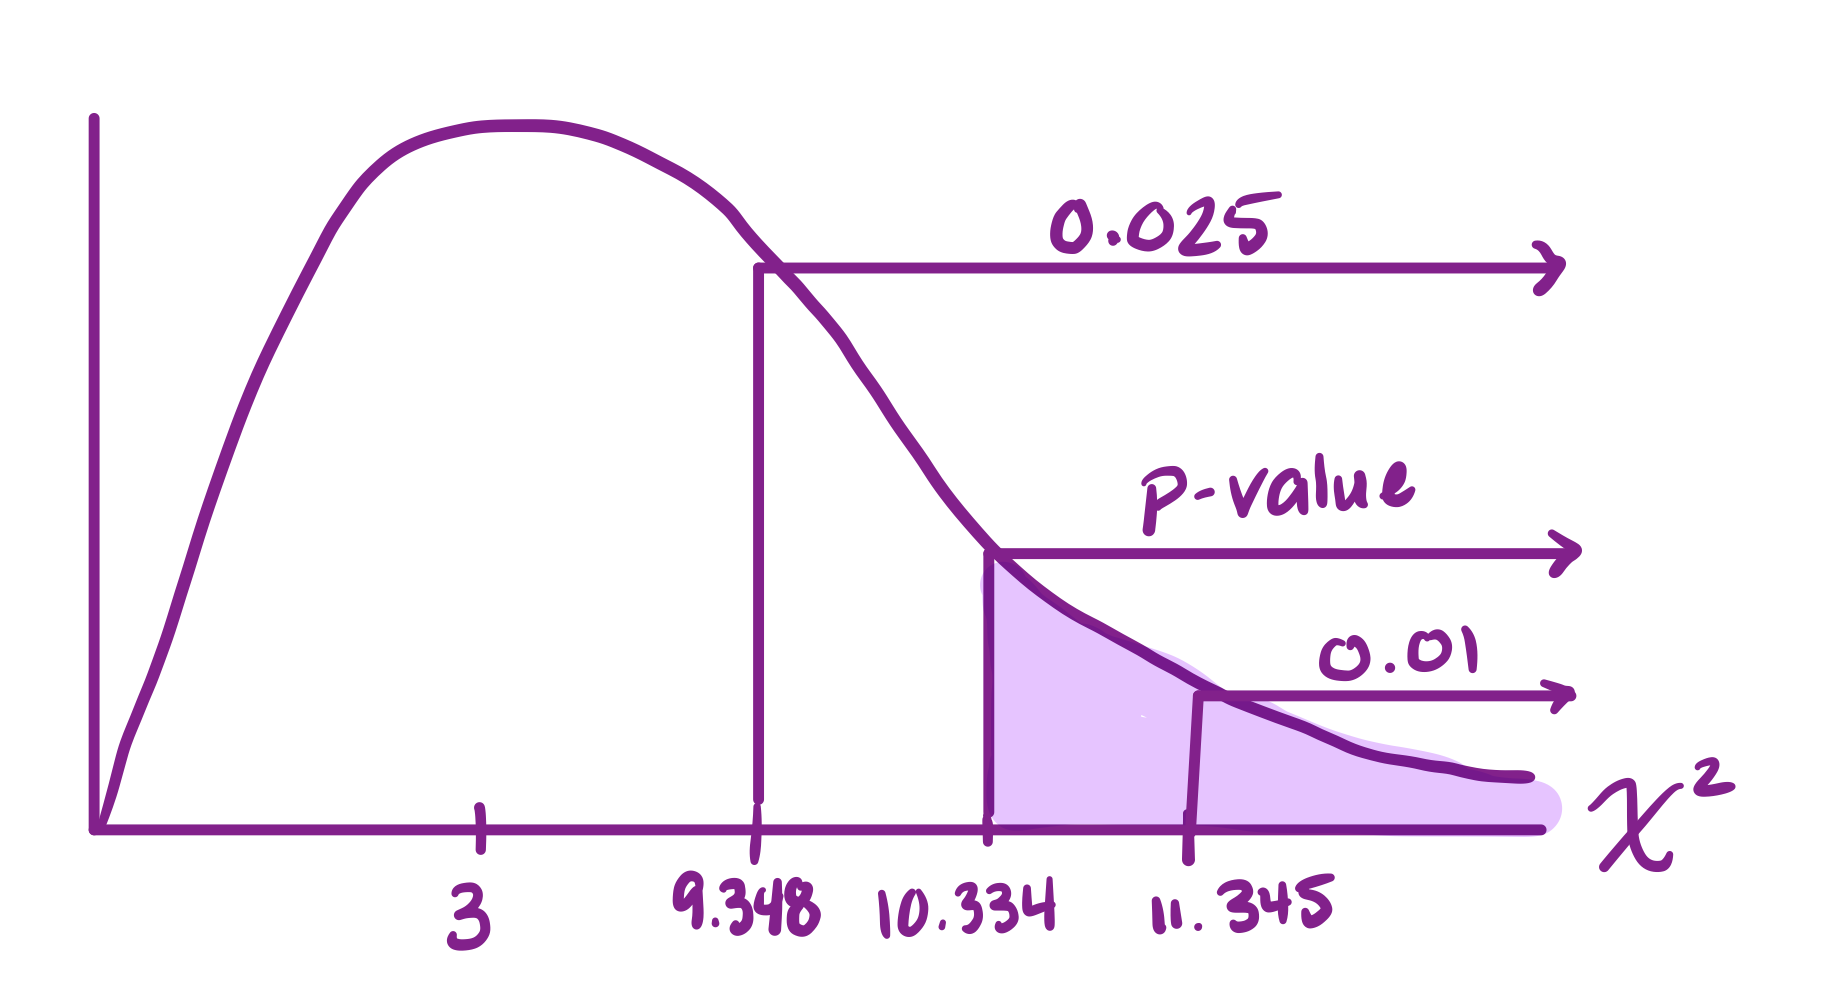
\includegraphics[scale=0.09]{STAT_2300_Practice_12-2_ChiSquare.JPEG}

\vspace{3mm}

\end{solution}

\part What is the \textbf{exact p-value} from your JMP output?

\begin{solution}[\stretch{1}]

\vspace{3mm}

p-value $=0.0159$

\vspace{3mm}

\end{solution}

\part State your \textbf{conclusion} in context.

\begin{solution}[\stretch{1}]

\vspace{3mm}

Reject $H_0$ because the p-value is smaller than $\alpha=0.05$. At the 5\% level, there is sufficient evidence that gender and highest degree earned are dependent.

\vspace{3mm}

\end{solution}

\end{parts}

\newpage

\question The following data were compiled on medals won by different countries in several years of the Olympics. 

\begin{center}
\begin{tabular}{|c|c|c|c|}
\hline
 & \textbf{Bronze} & \textbf{Silver} & \textbf{Gold}\\
 \hline
 \textbf{China} & 26 & 28 & 26 \\
 \hline
 \textbf{Great Britain} & 17 & 23 & 27 \\
 \hline
 \textbf{Russia} & 19 & 18 & 19 \\
 \hline
 \textbf{United States} & 38 & 37 & 46 \\
 \hline
 \textbf{Other} & 260 & 211 & 189 \\
 \hline 
\end{tabular}
\end{center}

Investigate whether there is an association between country and type of medal won. Use a significance level of $\alpha=0.05$.

\vspace{2mm}


\begin{parts}

\part State the appropriate \textbf{hypotheses} in this context.

\begin{solution}[\stretch{1}]

\vspace{3mm}

$H_0$: Country and medal type are independent (not associated)

$H_1$: Country and medal type are dependent (associated)

\vspace{3mm}

\end{solution}

\part What is the \textbf{expected count} for gold medals from the United States?

\begin{solution}[\stretch{1}]

\vspace{3mm}

$E=\displaystyle\frac{\text{Row Total}\times\text{Column Total}}{\text{Total Sample Size}}=\frac{121\times 307}{984}=37.751$

\vspace{3mm}

\end{solution}

\part Are the \textbf{conditions} for the chi-square test of independence of gender and highest degree earned met?

\begin{solution}[\stretch{1}]

\vspace{3mm}

Yes, because all expected counts are greater than 5.

\vspace{3mm}

\end{solution}

\part Calculate the chi-square \textbf{test statistic}.

\begin{solution}[\stretch{1}]

\vspace{3mm}

$E=\displaystyle\frac{(26-29.2683)^2}{29.2683}+\dots+\frac{(37-38.9807)^2}{38.9807}=10.631$ (from output)

\vspace{3mm}

\end{solution}

\part Find the \textbf{approximate p-value} using the chi-square table. Include a sketch.

\begin{solution}[\stretch{1}]

\vspace{3mm}

$df=(r-1)(c-1)=(5-1)(3-1)=(4)(2)=8$  \hspace{20mm} p-value $>0.10$

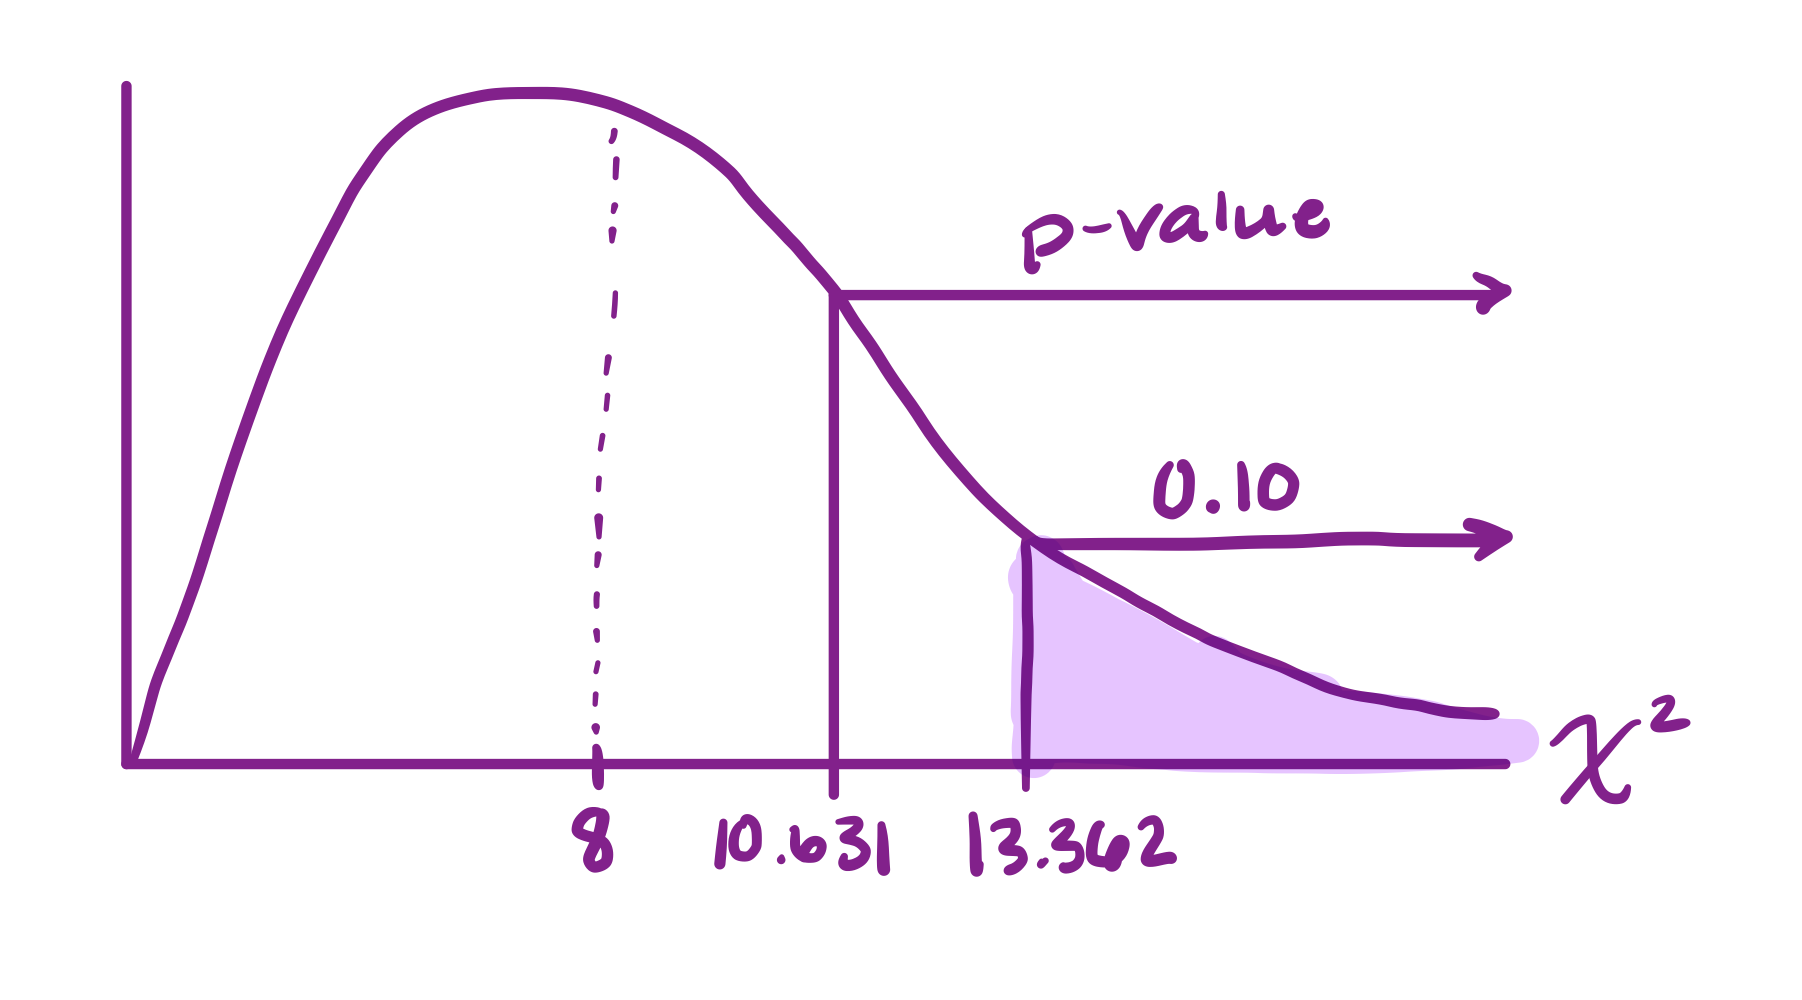
\includegraphics[scale=0.09]{STAT_2300_Practice_12-2_ChiSquare2.JPEG}

\vspace{3mm}

\end{solution}

\part What is the \textbf{exact p-value} from your JMP output?

\begin{solution}[\stretch{1}]

\vspace{3mm}

p-value $=0.2235$

\vspace{3mm}

\end{solution}

\part State your \textbf{conclusion} in context.

\begin{solution}[\stretch{1}]

\vspace{3mm}

Do not reject $H_0$ because the p-value is larger than $\alpha=0.05$. At the 5\% level, there is insufficient evidence that country and medal type in the Olympics are dependent.

\newpage 

For reference, your JMP output for \#2 should be as follows.

\vspace{3mm}

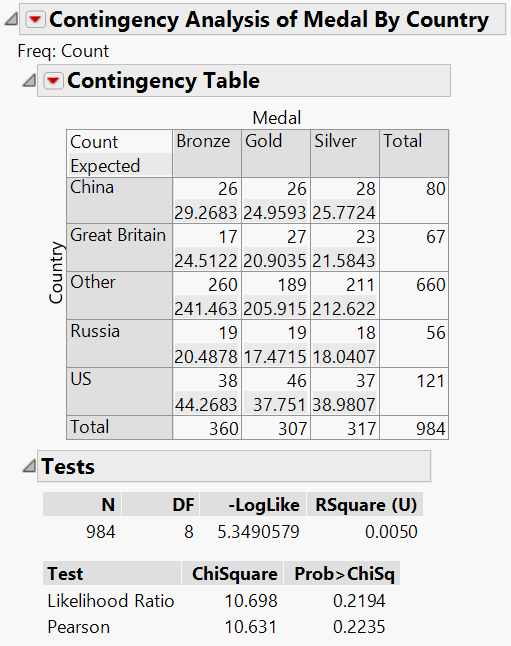
\includegraphics[scale=1]{STAT_2300_Practice_12-2_JMP.PNG}

\end{solution}

\end{parts}

\end{questions}
%-----------------------------------------------------------------------------%

\end{document}
